\section{Fundamentals} \label{sec:fundamentals}
In this section, I outline the necessary background for my research. I begin by providing a general overview of keyword mnemonics and their benefits for memory retention. Next, I discuss the application of mnemonics in learning Japanese Kanji, focusing on the unique challenges posed by this writing system. Lastly, I explore AI generation methods that are particularly suited for creating mnemonics and highlight the absence of a simple evaluation method to optimize this process.
\subsection{Keyword Mnemonics}
The world record in recalling historic dates is roughly equal to all the dates children have to learn during their entire time in school. The world record holder memorized them in five minutes while the average high-school student, looking back on their 12 years of education, is likely to remember no more than a handful of them \cite{how_to_become_a_memory_master}. It took Zou Lujian 13.96 seconds to remember the order of a shuffled deck of 52 playing cards \cite{record_recall_playing_cards}.

The incredible success of mnemonic devices can be traced back far beyond the Ancient Greeks \cite{white_2014}. Simonides allegedly helped to identify bodies of a collapsed building as he had remembered every person in a large banquet hall of the building by using a mnemonic device that we call today: \emph{loci}. As the word loci suggests, it works by imagining a familiar place in one's mind and associating parts of that place with things one wants to remember.

There are numerous mnemonic devices suited for various tasks such as Peg lists, acronyms and phonetic systems. They can be used for simple things like remembering a shopping list or phone number. Skilled memory athletes optimize them to remember up to 70.000 decimal places of PI \cite{record_decimal_pi}. 

Relevant for my research is the \emph{keyword mnemonic} that steps out of the memory athlete realm and shines with more practical applications most commonly found in second language learning. The process involves finding a keyword that is phonetically similar to the one the student wants to learn and then form a sentence or phrase that connects the two words in a meaningful manner. E.g. the Japanese word 食べる (taberu) meaning \emph{to eat} sounds like the word \emph{table}. Following one could come up with a mnemonic phrase like so: "Imagine you eat your lunch on the table. You wouldn't eat on the floor. That's inappropriate!". 

\subsection{Japanese Kanji}
Keyword mnemonics can be applied to Japanese Kanjis. The Japanese written language includes thousands of so called Kanjis. These are complex characters, that are composed of simpler parts called Radicals. There are just a few hundreds of those. Given one has a solid memory of the Radicals, it is easy to identify them in Kanjis.

In my earlier example of keyword mnemonics the meaning of the foreign word 食べる (taberu) was triggered by the keyword \emph{table}, because of their phonetic similarity. With Kanjis we are given the keywords by their Radicals instead. The clue in this case is visual rather than phonetic. Based on the meaning of a Kanji's Radicals one creates a mnemonic that connects them with the meaning of the Kanji. I have provided an example of this in Figure \ref{figure:robanohashi_example}.

\begin{figure}
    \centering
    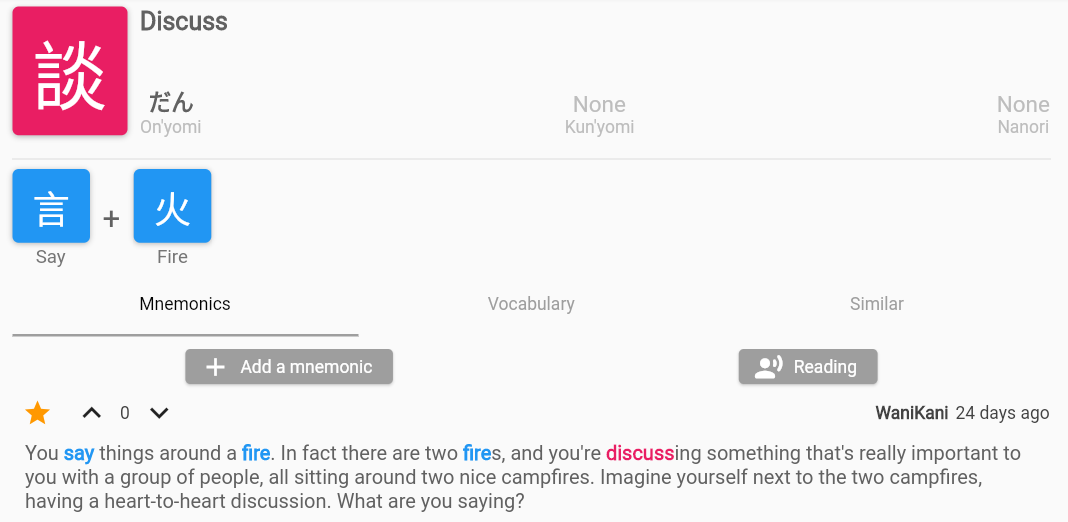
\includegraphics[width=400pt]{resources/robanohashi_example.png}
    \caption{This is a screenshot of \emph{robanohashi.org} show casing the application of keyword mnemonics for Japanese Kanjis.}
    \label{figure:robanohashi_example}
\end{figure}
This application of keyword mnemonics has been implemented at scale by a website called WaniKani \cite{wanikani}. 

\subsection{AI generation}
Despite the incredible success of mnemonics among memory athletes, they are mostly absent in the classroom. As has been pointed out by \cite{putnam_2015} one of the reasons for this is due to the time it takes to learn the techniques and subsequently apply them to create mnemonics. This gap has been closed by the aforementioned website Wankani as they account for the latter. 

The website allows students to learn the most common 1700 Kanjis, each accompanied by a hand-crafted mnemonic. It may be argued that bypassing that step of individual mnemonic creation reduces the memory retention of the Kanjis as students do not go through the work of creation themselves. However, \cite{campos_2004} has shown that there was no significant difference between groups that learned with mnemonics created by experts compared to groups that utilized subject-generated mnemonics.

Recent developments in Artificial Intelligence yielded ground-breaking, highly-capable language models. We can use those to create mnemonics to extend the existing ones, created by e.g. WaniKani. Moreover, the AI generated mnemonics can be tailored to individuals to account for differences in relatability of mnemonics among students. 

In order to assess model performance and for further model optimization it is necessary to have ways that can evaluate the model output. This is no different with the use case of generating mnemonics. The process is visualized in Figure \ref{figure:overall_process}.
\begin{figure}
    \centering
    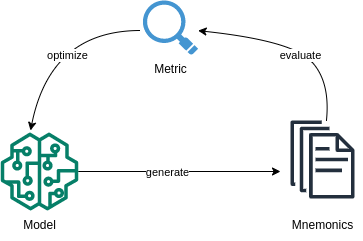
\includegraphics[width=300pt]{resources/general.png}
    \caption{A diagram visualizing the process of generating mnemonics with AI language models, evaluating their quality and in turn optimizing the model}
    \label{figure:overall_process}
\end{figure}


There are numerous language model architectures and generation techniques that could be used for the generation step. Research on these topics is abundant. Moreover, the outlined process in Figure \ref{figure:overall_process} remains the same, independent of the chosen generation model or technique. In any case we need a way to evaluate the output. In the highly specific case of generating keyword mnemonics for Japanese Kanjis there is no straightforward option available. Hence I have focused my research on that crucial step.  

Before concluding this chapter I want to briefly touch on one AI generation technique, since it has been used extensively throughout my research and is a powerful and cost-efficient way to begin. Increasingly complex language models are capable of zero-shot task transfers \cite{radford2019language}. This ability of fulfilling tasks, models have not specifically been trained on, led to a new field that aims to produce the best output given an optimal task description to the model. This field is most commonly known as \emph{prompt engineering}. Just like with any other generation method, the output needs to be evaluated to find an optimal prompt.